% VS Code (LaTeX Workshop) ayarlarının (output klasörü ve synctex) devreye girmesi için !TeX program satırları kaldırıldı.
\documentclass[light]{lutbeamer}

\usepackage{pgfpages}
\usepackage{ragged2e}
\usepackage{booktabs}
\usepackage{amssymb}
\usepackage{fontawesome5}
\usepackage{tikz}
\usepackage{pgfplots}
\pgfplotsset{compat=1.18}
\addbibresource{references.bib}

% ===================================================================
% METADATA (DERS KIMLIK BILGILERI)
% ===================================================================
\setdepartment{OSTIM Teknik Üniversitesi}
\institute{}
\author[Mühendislik Fakültesi]{\\Prof.~Dr.~Yalçın ATA,\\ 
Prof.~Dr.~Arif DEMİR,\\ Dr.~Öğr.~Üyesi~Emel GÜVEN,\\ Dr.~Öğr.~Üyesi~Ufuk ASIL,\\ Dr.~Öğr.~Üyesi~Haydar KILIÇ,\\ Dr.~Öğr.~Üyesi~Muhammed ELMNEFİ,\\ Öğr.~Gör.~Sema ÇİFTÇİ}
\title{MATH 204 -- Olasılık ve İstatistik}
\subtitle{Hafta 5: Beklenen Değer ve Varyans}
\date{2025--2026 Bahar Dönemi}

% ===================================================================
% AUTOMATIC TABLE OF CONTENTS (PRESENTATION FLOW)
% ===================================================================
\setcounter{tocdepth}{2}

\AtBeginSection[]{
  \begin{frame}{Sunum Planı}
    \scriptsize
    \begin{columns}[T]
      \begin{column}{0.48\textwidth}
        \tableofcontents[sections={1,2}, currentsection]
      \end{column}
      \begin{column}{0.48\textwidth}
        \tableofcontents[sections={3,4,5,6,7,8,9,10}, currentsection]
      \end{column}
    \end{columns}
  \end{frame}
}

\begin{document}

\setbeamertemplate{navigation symbols}{}
\setbeamertemplate{footline}{
  \begin{beamercolorbox}[wd=\paperwidth, ht=10pt, dp=1pt]{footline}
    \usebeamerfont{footline}
    \begin{tikzpicture}[remember picture,overlay]
      \node[anchor=south west, xshift=10mm, yshift=.4mm]
      at (current page.south west)
      {\insertshortauthor,~\department};
    \end{tikzpicture}
    \begin{tikzpicture}[remember picture,overlay]
      \node[anchor=south east, xshift=-5mm, yshift=0.5mm]
      at (current page.south east)
      {\insertframenumber \,/\, \inserttotalframenumber};
    \end{tikzpicture}
  \end{beamercolorbox}
}

% ===================================================================
% KAPAK SLAYTLARI
% ===================================================================

% Gorsel Tam Kapak (Logosuz)
\begin{frame}<article:0>[plain,noframenumbering]
  \begin{tikzpicture}[remember picture,overlay]
    \node[anchor=center, at=(current page.center), inner sep=0pt] {
      \includegraphics[width=\paperwidth, height=\paperheight]{logos/background_figure.jpg}
    };
  \end{tikzpicture}
\end{frame}

% Resmi Baslik Sayfasi (kapak icin ozel alt bilgi)
{
  \setbeamertemplate{footline}{
    \begin{beamercolorbox}[wd=\paperwidth, ht=10pt, dp=1pt]{footline}
      \usebeamerfont{footline}
      \begin{tikzpicture}[remember picture,overlay]
        \node[anchor=south west, xshift=10mm, yshift=.4mm, align=left]
        at (current page.south west)
        {\tiny Bu şablon OTU Yazılım Mühendisliği tarafından hazırlanmış olup \href{https://github.com/ufukasia/Ostim-Teknik--niversitesi-Yaz-l-m-M-hendisli-i---Lutbeamer-egitim-i-eri-i-haz-rlama-}{buradan} güncel haline ulaşabilirsiniz.};
      \end{tikzpicture}
      \begin{tikzpicture}[remember picture,overlay]
        \node[anchor=south east, xshift=-5mm, yshift=0.5mm]
        at (current page.south east)
        {\insertframenumber \,/\, \inserttotalframenumber};
      \end{tikzpicture}
    \end{beamercolorbox}
  }
  \maketitle{}
}

% GENEL ICERIK HARITASI
\begin{frame}{İçindekiler}
  \scriptsize
  \begin{columns}[T]
    \begin{column}{0.48\textwidth}
      \tableofcontents[sections={1,2}]
    \end{column}
    \begin{column}{0.48\textwidth}
      \tableofcontents[sections={3,4,5,6,7,8,9,10}]
    \end{column}
  \end{columns}
\end{frame}

% -------------------------------------------------------------------
% 0. İKONİK ÖRNEK: ORTALAMA VE VARYANS (ATIŞ TAHTASI)
% -------------------------------------------------------------------
\begin{frame}{İkonik Örnek: Polis Akademisi Atış Eğitimi}
  \justifying{}
  \small \textbf{Vaka:} Bir polis akademisinde 4 farklı polis memurunun (A, B, C, D) silah eğitimindeki atış sonuçları aşağıdaki hedef kağıtlarında verilmiştir. Her memur kendi beylik tabancasıyla hedefe 5'er atış yapmıştır.

  \vspace{0.4em}
  \centering
  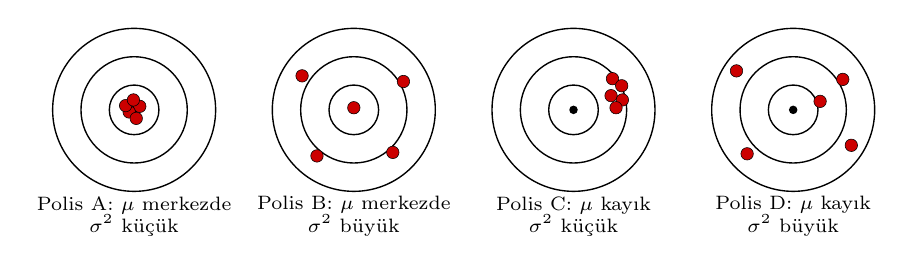
\begin{tikzpicture}[scale=0.9]
    \tikzset{
      board/.style={line width=0.5pt},
      shot/.style={fill=red!80!black, draw=black, line width=0.2pt}
    }

    % A: Dogru ortalama, dusuk varyans (iyi kalibrasyon + iyi hassasiyet)
    \draw[board] (-4.6,1.6) circle (1.15);
    \draw[board] (-4.6,1.6) circle (0.75);
    \draw[board] (-4.6,1.6) circle (0.35);
    \fill[black] (-4.6,1.6) circle (0.06);
    \node[shot] at (-4.52,1.65) [circle, minimum size=4.5pt, inner sep=0pt] {};
    \node[shot] at (-4.67,1.57) [circle, minimum size=4.5pt, inner sep=0pt] {};
    \node[shot] at (-4.57,1.48) [circle, minimum size=4.5pt, inner sep=0pt] {};
    \node[shot] at (-4.72,1.66) [circle, minimum size=4.5pt, inner sep=0pt] {};
    \node[shot] at (-4.61,1.74) [circle, minimum size=4.5pt, inner sep=0pt] {};
    \node[align=center, font=\scriptsize] at (-4.6,0.1) {Polis A: $\mu$ merkezde\\$\sigma^2$ küçük};

    % B: Dogru ortalama, yuksek varyans (iyi kalibrasyon + kotu hassasiyet)
    \draw[board] (-1.5,1.6) circle (1.15);
    \draw[board] (-1.5,1.6) circle (0.75);
    \draw[board] (-1.5,1.6) circle (0.35);
    \fill[black] (-1.5,1.6) circle (0.06);
    \node[shot] at (-2.23,2.08) [circle, minimum size=4.5pt, inner sep=0pt] {};
    \node[shot] at (-0.80,2.00) [circle, minimum size=4.5pt, inner sep=0pt] {};
    \node[shot] at (-2.02,0.95) [circle, minimum size=4.5pt, inner sep=0pt] {};
    \node[shot] at (-0.95,1.00) [circle, minimum size=4.5pt, inner sep=0pt] {};
    \node[shot] at (-1.50,1.63) [circle, minimum size=4.5pt, inner sep=0pt] {};
    \node[align=center, font=\scriptsize] at (-1.5,0.1) {Polis B: $\mu$ merkezde\\$\sigma^2$ büyük};

    % C: Kayik ortalama, dusuk varyans (sistematik hata + iyi hassasiyet)
    \draw[board] (1.6,1.6) circle (1.15);
    \draw[board] (1.6,1.6) circle (0.75);
    \draw[board] (1.6,1.6) circle (0.35);
    \fill[black] (1.6,1.6) circle (0.06);
    \node[shot] at (2.15,2.04) [circle, minimum size=4.5pt, inner sep=0pt] {};
    \node[shot] at (2.28,1.94) [circle, minimum size=4.5pt, inner sep=0pt] {};
    \node[shot] at (2.13,1.80) [circle, minimum size=4.5pt, inner sep=0pt] {};
    \node[shot] at (2.29,1.74) [circle, minimum size=4.5pt, inner sep=0pt] {};
    \node[shot] at (2.20,1.63) [circle, minimum size=4.5pt, inner sep=0pt] {};
    \node[align=center, font=\scriptsize] at (1.6,0.1) {Polis C: $\mu$ kayık\\$\sigma^2$ küçük};

    % D: Kayik ortalama, yuksek varyans (hem bias hem daginiklik)
    \draw[board] (4.7,1.6) circle (1.15);
    \draw[board] (4.7,1.6) circle (0.75);
    \draw[board] (4.7,1.6) circle (0.35);
    \fill[black] (4.7,1.6) circle (0.06);
    \node[shot] at (3.90,2.15) [circle, minimum size=4.5pt, inner sep=0pt] {};
    \node[shot] at (5.40,2.03) [circle, minimum size=4.5pt, inner sep=0pt] {};
    \node[shot] at (4.05,0.98) [circle, minimum size=4.5pt, inner sep=0pt] {};
    \node[shot] at (5.52,1.10) [circle, minimum size=4.5pt, inner sep=0pt] {};
    \node[shot] at (5.08,1.72) [circle, minimum size=4.5pt, inner sep=0pt] {};
    \node[align=center, font=\scriptsize] at (4.7,0.1) {Polis D: $\mu$ kayık\\$\sigma^2$ büyük};
  \end{tikzpicture}

  \vspace{0.2em}
  \begin{exampleblock}{Soru}
    \footnotesize
    \begin{itemize}
      \item \textbf{Polis C}'nin durumu hakkında ne söyleyebilirsiniz? Polisin atıcılık yeteneği nasıldır, kullandığı beylik tabancasının nişangah ayarı hakkında ne tür bir yorum yapılabilir?
      \item Sadece tabancasının bakıma ihtiyacı olan polis ile yeniden atış eğitimine alınması gereken polis kimdir?
    \end{itemize}
  \end{exampleblock}
\end{frame}

\begin{frame}{Durum Analizi: Ortalama ve Varyans}
  \justifying{}
  \small Ortalama ($\mu$) \textbf{silahın nişangah ayarını} (merkezi), varyans ($\sigma^2$) ise \textbf{polisin atış hassasiyetini} (yayılımı) ölçer.

  \vspace{1em}
  Bu atış sonuçlarına göre; atışların ortalaması merkezden sapıyorsa silahın nişangahında \textbf{sistematik hata (bias)}, atışlar çok dağınıksa atıcıda \textbf{yüksek varyans (kararsızlık)} vardır.

  \vspace{1em}
  \textbf{İpucu:} En başarılı ve göreve tam hazır polis A'dır. Sahada en büyük riski taşıyan ise polis D'dir.
\end{frame}

% ===================================================================
% ICERIK: HAFTA 5 - BEKLENEN DEGER VE VARYANS
% ===================================================================

% -------------------------------------------------------------------
% 1. HİKAYE VE GÖRSEL (PROBLEM TANIMI)
% -------------------------------------------------------------------
\begin{frame}{Vaka Analizi: Kumarhane Matematiği (Rulet)}
    \begin{columns}[T]
        % SOL SÜTUN: Hikaye Metni
        \begin{column}{0.62\textwidth}
        \justifying{}
        \textbf{Bağlam/Gözlem:} \\
        Dünyadaki dev kumarhaneler misafirlerine ücretsiz içkiler, gösterişli odalar sunar ve binlerce dolar kaybeden oyunculara bile güler yüz gösterirler. Oyuncular bazen büyük ikramiyeyi (jackpot) kazansalar bile, kumarhane yönetimi asla endişelenmez.

        \vspace{0.8em}
        \textbf{Problem:} \\
        Bir oyuncunun rulet masasında ``Kırmızı'' renge 100~TL yatırdığını düşünelim. Kazanırsa 100~TL alır, kaybederse 100~TL'si gider.

        \vspace{0.8em}
        \textbf{Yanlış Algı:} \\
        Birçok insan, kazanma ihtimalinin $\%50$, kaybetme ihtimalinin $\%50$ olduğunu ve oyunun tamamen ``şansa'' dayalı adil bir oyun olduğunu düşünür.
        \end{column}
        % SAĞ SÜTUN: İkonik Görsel
        \begin{column}{0.35\textwidth}
        \centering
        \includegraphics[width=\linewidth, keepaspectratio]{figures/roulette_expected_value.png}
        \end{column}
    \end{columns}
\end{frame}

% -------------------------------------------------------------------
% 2. TARTIŞMA VE SORU (İNTERAKTİF)
% -------------------------------------------------------------------
\begin{frame}{Soru: Kasa Gerçekten Şanslı mı?}
    \justifying{}
    Bir Avrupa rulet çarkında 18 kırmızı, 18 siyah ve \textbf{1 tane yeşil (0)} bölme vardır (toplam 37 bölme).

    \vspace{1em}
    Eğer Kırmızı gelirse oyuncu $+100$~TL kazanır. Siyah veya Yeşil (0) gelirse oyuncu $-100$~TL kaybeder (kasa kazanır).
    
    \vspace{1em}
    \textbf{Genel Kanı:} \\
    \textit{``Oyuncu bazen üst üste kazanabilir, bazen kaybedebilir. Sonuçta şans kimden yanaysa o cebini doldurur ve büyük kazananlar kumarhaneyi batırabilir.''}

    \vspace{1.5em}
    \begin{exampleblock}{Mühendislik Sorusu:}
        Siz bir matematikçi veya süreç mühendisi olsaydınız, kumarhane müdürüne ``Bir oyuncunun tek bir tur oynamasının kumarhaneye parasal değeri (getirisi) kesin olarak nedir?'' sorusunu nasıl yanıtlardınız?
    \end{exampleblock}
\end{frame}

% -------------------------------------------------------------------
% 3. ÇÖZÜM VE DERS (BİLİMSEL GERÇEK)
% -------------------------------------------------------------------
\begin{frame}{Çözüm: Beklenen Değerin Acımasız Kanunu}
    \justifying{}
    Durumu bir \textbf{Rastgele Değişken ($X$)} olarak tanımlayalım. $X$, oyuncunun 1 eldeki kazancıdır.

    \vspace{0.5em}
    \begin{block}{Matematiksel Analiz}
        \begin{itemize}
            \item \textbf{Kazanma ($X = +100$~TL):} Olasılık $= \frac{18}{37}$
            \item \textbf{Kaybetme ($X = -100$~TL):} Olasılık $= \frac{19}{37}$ (18 siyah + 1 yeşil)
        \end{itemize}
        
        \vspace{0.5em}
        $\text{Ortalama Kazanç} = (+100) \cdot \left(\frac{18}{37}\right) + (-100) \cdot \left(\frac{19}{37}\right) = \mathbf{-2{,}70 \text{ TL}}$
    \end{block}

    \vspace{0.5em}
    \textbf{İstatistiksel Ders (Beklenen Değer):} Matematiksel olarak oyuncu masaya her oturduğunda, tekerlek hiç dönmeden oyuncunun cebinden kasaya teorik olarak \textbf{2,70~TL} geçmektedir. Kasa, kısa vadeli şansa (``varyans') değil, uzun vadeli garanti ortalamaya (``beklenen değer') yatırım yapar.
    \\ \vspace{0.5em} \centering
    \textit{İşte mühendislik ve fizikte de \textbf{Beklenen Değer}; rastgelelik içeren uzun vadeli süreçlerin nereye yakınsayacağının kesin ve acımasız yasasıdır.}
\end{frame}
% -------------------------------------------------------------------



\begin{frame}{Hafta 4'ten Ne Getiriyoruz?}
    \begin{block}{Temel Hatırlatma}
        Geçen hafta öğrendiğimiz kavramlar:
        \begin{itemize}
            \item Ayrık ve Sürekli \textbf{Rastgele Değişkenler} ($X, Y$).
            \item Olasılık Dağılımları (Olasılık Kütle/Yoğunluk Fonksiyonu $f(x)$).
            \item Olayların olasılıklarını sadece bir \textbf{fonksiyon denklemiyle} veya \textbf{tabloyla} tanımlamayı öğrendik.
        \end{itemize}
    \end{block}

    \begin{itemize}
        \item Dağılımları elde ettik ama bir dağılımın \textbf{karakterini} (merkezini ve yayılımını) tek bir sayıyla özetlemedik.
        \item \textbf{Bu hafta:} Bir olasılık dağılımının \textbf{ortalamasını} (Beklenen Değer) ve değerlerin bu ortalama etrafındaki \textbf{yayılımını} (Varyans/Standart Sapma) hesaplayıp analiz edeceğiz.
    \end{itemize}
\end{frame}

% ===================================================================
% KAVRAM HARITASI - KENDI KENDINE CALISMAYA UYGUN ACIKLAMALI
% ===================================================================
\begin{frame}{Kavram Haritası: Bu Hafta Neyi Ölçeceğiz?}
    \vspace{0.2cm}
    \centering
    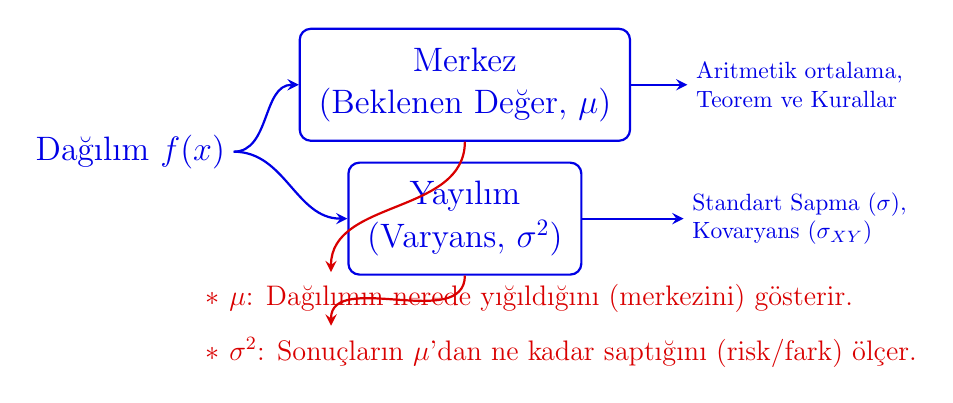
\begin{tikzpicture}[scale=0.85, transform shape, >=stealth, thick]

        % MAVI KALEM KISMI
        \node[text=blue!90!black, font=\Large] (dagilim) at (-4, 2) {Dağılım $f(x)$};
        \node[draw=blue!90!black, rounded corners, inner sep=8pt, text=blue!90!black, font=\Large, align=center] (merkez) at (1, 3) {Merkez\\(Beklenen Değer, $\mu$)};
        \node[draw=blue!90!black, rounded corners, inner sep=8pt, text=blue!90!black, font=\Large, align=center] (yayilim) at (1, 1) {Yayılım\\(Varyans, $\sigma^2$)};

        \node[text=blue!90!black, font=\normalsize, align=left] (ozellik1) at (6, 3) {Aritmetik ortalama,\\Teorem ve Kurallar};
        \node[text=blue!90!black, font=\normalsize, align=left] (ozellik2) at (6, 1) {Standart Sapma ($\sigma$),\\Kovaryans ($\sigma_{XY}$)};

        % Mavi Oklar
        \draw[->, blue!90!black] (dagilim.east) to[out=0, in=180] (merkez.west);
        \draw[->, blue!90!black] (dagilim.east) to[out=0, in=180] (yayilim.west);
        \draw[->, blue!90!black] (merkez.east) -- (ozellik1.west);
        \draw[->, blue!90!black] (yayilim.east) -- (ozellik2.west);

        % KIRMIZI/PEMBE KALEM KISMI
        \colorlet{mypink}{red!85!black}
        \node[text=mypink, font=\large, align=left, anchor=west] (prop1) at (-3, -0.2) {\textbf{$\ast$} $\mu$: Dağılımın nerede yığıldığını (merkezini) gösterir.};
        \node[text=mypink, font=\large, align=left, anchor=west] (prop2) at (-3, -1.0) {\textbf{$\ast$} $\sigma^2$: Sonuçların $\mu$'dan ne kadar saptığını (risk/fark) ölçer.};
        \draw[->, mypink] (merkez.south) to[out=270, in=90] (-1, 0.2);
        \draw[->, mypink] (yayilim.south) to[out=270, in=90] (-1, -0.6);
    \end{tikzpicture}

    \vspace{0.2cm}
    \begin{exampleblock}{Önemli Kılavuz Bilgi}
        \footnotesize İstatistikte veriyi tam bir tablo/grafik ile sunmak yerine, \textbf{Beklenen Değer} ve \textbf{Varyans} (veya Standart Sapma) gibi birkaç kritik ölçüye indirgeyerek özetleriz. Bu iki değer, farklı senaryoları (örneğin iki ayrı üretim hattını) \textbf{hızlı şekilde karşılaştırmak} için en iyi köprüdür.
    \end{exampleblock}
\end{frame}

\section{Beklenen Değer Kavramı}
\subsection{Beklenen Değerin Kavramsal Temeli}

\begin{frame}[fragile]
  \frametitle{Beklenen Değer (Matematiksel Beklenti) Nedir?}
  Bölüm~1'de verilerin aritmetik ortalaması olan \textbf{örneklem ortalamasından} (sample mean) bahsetmiştik. Şimdi aynı mantığı olasılık dağılımları üzerinden kuralım.

  \medskip
  İki madeni para 16 kez atılsın; $X$, her atışta elde edilen tura sayısı olsun. Deney sonucunda 4 defa sıfır, 7 defa bir ve 5 defa iki tura geldiğini varsayalım.
  \begin{columns}[T]
    \begin{column}{0.2\textwidth}
      \begin{block}{Dağılım Tablosu}
        \centering
        \scriptsize
        \begin{tabular}{@{}cc@{}}
          \toprule
          $x$ & Frekans \\
          \midrule
          0 & 4 \\
          1 & 7 \\
          2 & 5 \\
          \midrule
          Toplam & 16 \\
          \bottomrule
        \end{tabular}
      \end{block}
    \end{column}
    \begin{column}{0.75\textwidth}
      \begin{exampleblock}{Ortalama Tura Sayısı}
        \begin{center}
          $\bar{x} = \frac{(0)(4) + (1)(7) + (2)(5)}{16} = 1{,}06$
        \end{center}
      \end{exampleblock}
      \begin{itemize}
    \item Sonuç $1{,}06$, deneyin olası sonuçları \{0, 1, 2\} arasında \textbf{yer almaz}. Yani bir ortalama, her zaman gözlenebilir bir sonuç değildir.
    \item Benzer şekilde: Bir satış temsilcisinin aylık ortalama geliri, maaş çeklerinin hiçbirine tam olarak eşit olmayabilir.
  \end{itemize}
    \end{column}
  \end{columns}

\end{frame}

\begin{frame}[fragile]
  \frametitle[Göreceli Frekanslar]{Göreceli Frekanslardan Beklenen Değere}

  \justifying{}
  \small
  16 atışlık bu deneyde \textbf{gerçek olasılıkları} bilmiyoruz; elimizde sadece \textbf{gözlenen oranlar} var. Ortalamayı olasılık formuna benzetmek için göreceli frekansları ($\hat{p}$) kullanırız:

  \vspace{0.5em}
  \begin{columns}[T]
    \begin{column}{0.48\textwidth}
      \begin{block}{Gözlenen Durum ($n=16$)}
        \vspace{-1em}
        {\footnotesize
        \begin{align*}
          \hat{p}(0) &= \frac{4}{16},\; \hat{p}(1) = \frac{7}{16},\; \hat{p}(2) = \frac{5}{16} \\[0.5em]
          \bar{x} &= (0)\hat{p}(0) + (1)\hat{p}(1) + (2)\hat{p}(2) \\
                  &= 1{,}06
        \end{align*}
        }
      \end{block}
    \end{column}
    \begin{column}{0.48\textwidth}
      \begin{exampleblock}{Teorik Durum (Adil Para)}
        \vspace{-1em}
        {\footnotesize
        \begin{align*}
          P(X=0) &= \frac{1}{4},\; P(X=1) = \frac{1}{2},\; P(X=2) = \frac{1}{4} \\[0.5em]
          \mu &= (0)\frac{1}{4} + (1)\frac{1}{2} + (2)\frac{1}{4} \\
              &= 1
        \end{align*}
        }
      \end{exampleblock}
    \end{column}
  \end{columns}

  \vspace{0.5em}
  \begin{center}
    \begin{minipage}{0.98\textwidth}
      \footnotesize
      \textbf{Sonuç neden $\mathbf{1}$ çıkmadı?} Çünkü $n=16$ çok küçük bir örneklemdir ve kendi içinde rastgele dalgalanmalar barındırır. Deney sayısı arttıkça \textbf{göreceli frekanslar} teorik olasılıklara yaklaşır ve gözlenen örneklem ortalaması ($\bar{x}$) teorik beklenen değere ($\mu=1$) tam olarak yakınsar.
    \end{minipage}
  \end{center}
\end{frame}

\subsection{Kesikli ve Sürekli Değişkenlerde Beklenen Değer}

\begin{frame}[fragile]
  \frametitle{Tanım: Kesikli Rastgele Değişkenlerde Beklenen Değer}
  Herhangi bir kesikli rastgele değişkenin beklenen değerini bulmak için, her olası değeri kendi olasılığıyla çarpar ve toplarız.
  \begin{center}
    \begin{minipage}{0.9\textwidth}
      \begin{block}{Tanım 4.1 --- Kesikli Beklenen Değer}
        $X$, olasılık dağılımı $f(x)$ olan kesikli bir rastgele değişken olsun.
        \begin{center}
          $\mu = E(X) = \displaystyle\sum_{x} x\, f(x)$
        \end{center}
      \end{block}
    \end{minipage}
  \end{center}

  \medskip
  {\small \textbf{Dikkat:} Buradaki ortalama, Bölüm~1'deki \emph{örneklem ortalamasından} farklıdır. Örneklem ortalaması \textit{veriden}, beklenen değer ise \textit{olasılık dağılımından} hesaplanır. Beklenen değer, dağılımın ``merkez'' noktasını gösterir.}
\end{frame}

\begin{frame}[fragile]
  \frametitle[Örnek 4.1]{Örnek 4.1 --- Akıllı Telefon Kalite Kontrolü}

  \smallskip
  \begin{columns}[T,onlytextwidth]
    \begin{column}{0.49\textwidth}
      \footnotesize
      \textbf{Soru:} Bir teknoloji mağazasına gelen 7 cihazlık bir akıllı telefon
      koli/partisinde, 4 telefon sağlam (sorunsuz çalışmakta), 3 telefonun ise
      bataryası arızalıdır (kusurlu).

      \smallskip
      Kalite kontrol uzmanı, test etmek üzere rastgele 3 cihaz seçer.
      $X$, bu 3 cihazlık örneklemdeki sağlam telefon sayısıdır.
      Uzman ortalama kaç sağlam telefon tespit etmeyi bekler ($E(X)=?$)?


      \vspace{5em}
      \textbf{Yorum:} Örneklem başına ortalama
      $1{,}7$ sağlam telefon beklenir.
    \end{column}



    \begin{column}{0.49\textwidth}
      \footnotesize
      \vspace{-2.6em}
      \textbf{Çözüm:} Hipergeometrik dağılım:
      \[
      f(x)=\dfrac{\dbinom{4}{x}\dbinom{3}{3-x}}{\dbinom{7}{3}},
      \quad x=0,1,2,3
      \]
      \[
      f(0)=\tfrac{1}{35},\;
      f(1)=\tfrac{12}{35},\;
      f(2)=\tfrac{18}{35},\;
      f(3)=\tfrac{4}{35}
      \]
      \begin{align*}
        \mu=E(X)
        &= (0)\!\left(\tfrac{1}{35}\right)
         + (1)\!\left(\tfrac{12}{35}\right)
         + (2)\!\left(\tfrac{18}{35}\right)
         + (3)\!\left(\tfrac{4}{35}\right)\\
        &= \frac{12}{7}\approx 1{,}7
      \end{align*}
    \end{column}
  \end{columns}
\end{frame}

\begin{frame}[fragile]
  \frametitle[Örnek 4.2]{Örnek 4.2 --- Tıbbi Cihaz Satış Temsilcisi}

  \smallskip
  \textbf{Soru:} Tıbbi cihazlar satan bir satış temsilcisinin belirli bir günde iki randevusu vardır.
  İlk randevuda anlaşma yapma olasılığının $0{,}70$ olduğuna ve başarılı olursa $\$1000$ komisyon kazanacağına inanmaktadır. İkinci randevuda anlaşma yapma olasılığının sadece $0{,}40$ olduğunu düşünmekte ve başarılı olursa $\$1500$ kazanabileceğini öngörmektedir. 
  
  \medskip
  Randevu sonuçlarının bağımsız olduğu varsayımıyla, temsilcinin beklenen komisyonu nedir?
\end{frame}

\begin{frame}[fragile]
  \frametitle[Örnek 4.2]{Örnek 4.2 --- Tıbbi Cihaz Satış Temsilcisi}

  \setbeamercovered{transparent=7}
  \uncover<2->{
    {\color{red!80!black}
    \textbf{Çözüm:} Öncelikle temsilcinin toplam komisyonu ($X$) için 4 olası değer vardır: $\$0$, $\$1000$, $\$1500$ ve $\$2500$. Randevular bağımsız olduğundan, olasılıklar her durum için çarpılarak hesaplanır:
    {\small
    \begin{align*}
      f(\$0)    &= P(\text{İkisi de başarısız}) = (1 - 0{,}70)(1 - 0{,}40) = 0{,}18 \\
      f(\$1000) &= P(\text{Sadece ilk randevu başarılı}) = (0{,}70)(1 - 0{,}40) = 0{,}42 \\
      f(\$1500) &= P(\text{Sadece ikinci randevu başarılı}) = (1 - 0{,}70)(0{,}40) = 0{,}12 \\
      f(\$2500) &= P(\text{İkisi de başarılı}) = (0{,}70)(0{,}40) = 0{,}28
    \end{align*}
    }
    
    Kesikli rastgele değişkenler için beklenen değer formülü:
    \begin{equation*}
      E(X) = \sum_{x} x\, f(x)
    \end{equation*}

    Buna göre, formülü uyguladığımızda beklenen komisyon değeri:
    {\small
    \begin{align*}
      E(X) &= (\$0)(0{,}18) + (\$1000)(0{,}42) + (\$1500)(0{,}12) + (\$2500)(0{,}28) \\
           &= \$0 + \$420 + \$180 + \$700 
           &= \mathbf{\$1300}
    \end{align*}
    }
    }
  }
\end{frame}

\begin{frame}[fragile]
  \frametitle{Sürekli Rastgele Değişkenlerde Beklenen Değer}
  Sürekli durumda toplam yerini integral alır; mantık aynıdır.
  \begin{center}
    \begin{minipage}{0.9\textwidth}
      \begin{block}{Teorem 4.1 --- Sürekli Beklenen Değer}
        $X$, olasılık yoğunluk fonksiyonu $f(x)$ olan sürekli bir rastgele değişken olsun.
        \begin{center}
          $\mu = E(X) = \displaystyle\int_{-\infty}^{\infty} x\, f(x) \,dx$
        \end{center}
      \end{block}
    \end{minipage}
  \end{center}
\end{frame}

\begin{frame}[fragile]
  \frametitle[Örnek 4.3]{Örnek 4.3 --- Elektronik Cihaz Ömrü}

  \smallskip
  \textbf{Soru:} Belirli bir elektronik cihazın ömrü $X$ (saat), aşağıdaki yoğunluk fonksiyonuyla modelleniyor. Beklenen ömrü bulunuz.
  \begin{center}
    $f(x) = \begin{cases} \dfrac{20000}{x^3}, & x > 100 \\[4pt] 0, & \text{diğer durumlarda} \end{cases}$
  \end{center}

  \textbf{Çözüm:}
  {\small
  \begin{align*}
    \mu = E(X) &= \int_{100}^{\infty} x \cdot \frac{20000}{x^3} \,dx = \int_{100}^{\infty} \frac{20000}{x^2} \,dx \\[4pt]
               &= \left[ -\frac{20000}{x} \right]_{100}^{\infty} = 0 - \!\left(-\frac{20000}{100}\right) = 200 \text{ saat}
  \end{align*}
  }
  \textbf{Yorum:} Bu tip cihazların \textbf{ortalama ömrü 200 saat} olarak beklenir.
\end{frame}

\begin{frame}[fragile]
  \frametitle[Örnek 4.3 PDF]{Örnek 4.3 --- PDF Geçerlilik Kontrolü}
  {\small Bir fonksiyonun olasılık yoğunluk fonksiyonu (PDF/PDF) olabilmesi için iki koşulu sağlaması gerekir:}

  \begin{columns}[t,onlytextwidth]
    \begin{column}{0.48\textwidth}
      \begin{block}{PDF Koşulları}
        {\footnotesize
        \begin{enumerate}
          \item $f(x) \geq 0$ \quad tüm $x$ için
          \item $\displaystyle\int_{-\infty}^{\infty} f(x)\,dx = 1$
        \end{enumerate}
        }
      \end{block}

      {\footnotesize
      \textbf{Koşul 1 --- Negatif Olmama:}\\
      $x > 100$ için $x^3 > 0$ olduğundan
      $f(x) = \dfrac{20000}{x^3} > 0$.\\
      Diğer bölgelerde $f(x)=0 \geq 0$. \checkmark
      }
    \end{column}

    \begin{column}{0.48\textwidth}
      {\footnotesize
      \textbf{Koşul 2 --- Alan = 1:}
      \begin{align*}
        \int_{-\infty}^{\infty} f(x)\,dx
          &= \int_{100}^{\infty} \frac{20000}{x^3}\,dx \\
          &= 20000 \left[\frac{x^{-2}}{-2}\right]_{100}^{\infty} \\
          &= 20000 \cdot \frac{1}{2 \cdot 100^{2}}
           = \frac{20000}{20000}
           = \mathbf{1} \quad \checkmark
      \end{align*}

      Her iki koşul da sağlandığından $f(x)$, geçerli bir olasılık yoğunluk fonksiyonudur.
      }
    \end{column}
  \end{columns}
\end{frame}

\subsection{Fonksiyonların Beklenen Değeri}

\begin{frame}[fragile]
  \frametitle[Teorem 4.1]{$g(X)$ Fonksiyonunun Beklenen Değeri}
  Bazen doğrudan $X$ yerine, $X$'e bağlı bir fonksiyon $g(X)$'in beklenen değeriyle ilgileniriz (örn.\ $g(X) = X^2$, $g(X) = 2X-1$). Her seferinde $g(X)$'in dağılımını bulmak yerine şu pratik teorem kullanılır:
  \begin{center}
    \begin{minipage}{0.9\textwidth}
      \begin{block}{Teorem 4.1}
        {\small
        \begin{align*}
          E[g(X)] &= \sum_x g(x)\, f(x) \quad \text{(kesikli)} \\[4pt]
          E[g(X)] &= \int_{-\infty}^{\infty} g(x)\, f(x) \,dx \quad \text{(sürekli)}
        \end{align*}
        }
      \end{block}
    \end{minipage}
  \end{center}
  Bu teorem, $g(X)$'in olasılık dağılımını ayrıca türetmeye gerek kalmadan doğrudan $X$'in dağılımıyla işlem yapmamızı sağlar.
\end{frame}

\begin{frame}[fragile]
  \frametitle[Örnek 4.4]{Örnek 4.4 --- Otopark Yıkayıcısı Geliri}

  \smallskip
  \textbf{Soru:} Güneşli bir cuma 16:00--17:00 arası oto yıkamaya gelen araç sayısı $X$'in dağılımı aşağıdadır. Görevlinin geliri $g(X) = 2X - 1$ (\$). Beklenen geliri bulunuz.

  {\small
  \begin{center}
    \renewcommand{\arraystretch}{1.2}
    \begin{tabular}{ccccccc}
      \toprule
      $\mathbf{x}$ & 4 & 5 & 6 & 7 & 8 & 9 \\
      \midrule
      $\mathbf{g(x)=2x-1}$ & 7 & 9 & 11 & 13 & 15 & 17 \\
      \midrule
      $\mathbf{f(x)}$ & $\frac{1}{12}$ & $\frac{1}{12}$ & $\frac{1}{4}$ & $\frac{1}{4}$ & $\frac{1}{6}$ & $\frac{1}{6}$ \\
      \bottomrule
    \end{tabular}
  \end{center}
  }

  \textbf{Çözüm (Teorem 4.1):}
  {\small
  \begin{align*}
    E(2X\!-\!1) &= (7)\!\left(\tfrac{1}{12}\right) + (9)\!\left(\tfrac{1}{12}\right) + (11)\!\left(\tfrac{1}{4}\right) + (13)\!\left(\tfrac{1}{4}\right) + (15)\!\left(\tfrac{1}{6}\right) + (17)\!\left(\tfrac{1}{6}\right) \\
                &= \$12{,}67
  \end{align*}
  }
\end{frame}

\begin{frame}[fragile]
  \frametitle[Örnek 4.5]{Örnek 4.5 --- Fonksiyonun Beklenen Değeri}

  \smallskip
  \textbf{Soru:} $X$ rastgele değişkeninin yoğunluk fonksiyonu
  \[
    f(x)=
    \begin{cases}
      \dfrac{x^2}{3}, & -1<x<2,\\[2pt]
      0, & \text{diğer durumlarda}
    \end{cases}
  \]
  olsun. $E(4X+3)$ değerini bulunuz.

  \medskip
  \textbf{Çözüm (Teorem 4.1):}
  \[
    \int_{-1}^{2}\frac{x^2}{3}\,dx = 1,\qquad f(x)\ge 0
  \]
  \begin{align*}
    E(4X+3) &= \int_{-1}^{2} (4x+3)\,\frac{x^2}{3}\,dx = \frac{1}{3}\int_{-1}^{2}\bigl(4x^3 + 3x^2\bigr)\,dx = 8
  \end{align*}
\end{frame}


\begin{frame}[fragile]
  \frametitle{Varyansın Beklenen Değerle İlişkisi}
  Teorem~4.1 yalnızca basit fonksiyonlarda değil, daha ileri istatistiksel ölçülerin hesabında da kullanılır.

  \medskip
  Özel olarak $g(X) = (X - \mu)^2$ seçersek, $X$'in ortalamasından sapmalarının karesinin beklenen değerini elde ederiz:
  \begin{center}
    \begin{minipage}{0.7\textwidth}
      \begin{block}{Varyans --- Ön Tanım}
        \begin{center}
          $Var(X) = \sigma^2 = E\bigl[(X-\mu)^2\bigr]$
        \end{center}
      \end{block}
    \end{minipage}
  \end{center}
  Bu değer, verilerin ortalaması etrafındaki \textbf{yayılımın} (değişkenliğin) ölçüsüdür. Bir sonraki bölümde ayrıntılı olarak ele alınacaktır.
\end{frame}

% ─── SORULAR ─────────────────────────────────────
\subsection{Sorular}

\begin{frame}{Yeni Teknoloji Yatırımı}
  \textbf{\small $\triangleright$~Kesikli Beklenen Değer --- Olası Senaryo Analizi}

  \smallskip
  \small
  Bir teknoloji şirketi, yeni bir donanım üretim hattı kurmayı planlamaktadır. Piyasa araştırmalarına göre uygulamanın başarı senaryoları ve net kazanç/zarar ($-$ işareti zararı gösterir) durumları aşağıda verilmiştir:
  \begin{itemize}
    \item Çok başarılı olma olasılığı: $0{,}20$ (Kazanç: $\$50.000$)
    \item Orta düzeyde tutunma olasılığı: $0{,}50$ (Kazanç: $\$10.000$)
    \item Başarısız olma olasılığı: $0{,}30$ (Zarar: $-\$20.000$)
  \end{itemize}

  \medskip
  \begin{block}{Görev}
    $X$ rastgele değişkeni projenin net getirisini göstersin. Bu projenin \textbf{beklenen değerini} ($E(X)$) hesaplayınız ve yatırımın uzun vadeli mantığını yorumlayınız.
  \end{block}
\end{frame}

\begin{frame}{Yeni Teknoloji Yatırımı}
  \setbeamercovered{transparent=7}
  \uncover<2->{
    \small
    {\color{red!80!black}
      \textbf{Çözüm (Beklenen Değer):}

      Değerleri ve olasılıkları eşleştirelim:
      \begin{align*}
        x_1 &= 50.000, & f(x_1) &= 0{,}20 \\
        x_2 &= 10.000, & f(x_2) &= 0{,}50 \\
        x_3 &= -20.000, & f(x_3) &= 0{,}30
      \end{align*}

      Beklenen değeri formüle koyarsak:
      \begin{align*}
        E(X) &= (50.000)(0{,}20) + (10.000)(0{,}50) + (-20.000)(0{,}30) \\
             &= 10.000 + 5.000 - 6.000 \\
             &= \mathbf{\$9.000}
      \end{align*}
      
      \textbf{Yorum:} Projenin beklenen değeri pozitif ($\$9.000$) olduğundan, istatistiksel açıdan bu yatırım \textbf{karlıdır ve mantıklıdır}.
    }
  }
\end{frame}

\begin{frame}{$E(X)$ ve $E(X^2)$ Hesabı}
  \textbf{\small $\triangleright$~Kesikli Beklenen Değer --- $E(X)$ ve $E(X^2)$ Hesabı}

  \smallskip
  \small
  10~metrelik sentetik kumaştaki kusur sayısı $X$'in olasılık dağılımı:

  \medskip
  \begin{center}
    \renewcommand{\arraystretch}{1.2}
    \begin{tabular}{cccccc}
      \toprule
      $x$ & 0 & 1 & 2 & 3 & 4 \\
      \midrule
      $f(x)$ & 0{,}41 & 0{,}37 & 0{,}16 & 0{,}05 & 0{,}01 \\
      \bottomrule
    \end{tabular}
  \end{center}

  \medskip
  \begin{block}{Görev}
    \begin{enumerate}
      \item[(a)] $E(X)$, yani ortalama kusur sayısını hesaplayınız.
      \item[(b)] $E(X^2)$ değerini bulunuz.
    \end{enumerate}
  \end{block}
\end{frame}

\begin{frame}{$E(X)$ ve $E(X^2)$ Hesabı}
  \setbeamercovered{transparent=7}
  \uncover<2->{
    \small
    {\color{red!80!black}
      \textbf{(a) Beklenen Değer $E(X)$:}
      \begin{align*}
        E(X) &= (0)(0{,}41) + (1)(0{,}37) + (2)(0{,}16) + (3)(0{,}05) + (4)(0{,}01) \\
             &= 0 + 0{,}37 + 0{,}32 + 0{,}15 + 0{,}04 = \mathbf{0{,}88} \text{ kusur/10~m}
      \end{align*}

      \textbf{(b) $E(X^2)$ değeri:}
      \begin{align*}
        E(X^2) &= (0)(0{,}41) + (1)(0{,}37) + (4)(0{,}16) + (9)(0{,}05) + (16)(0{,}01) \\
               &= 0 + 0{,}37 + 0{,}64 + 0{,}45 + 0{,}16 = \mathbf{1{,}62}
      \end{align*}

      {\small \textit{Not: Bu değerleri bir sonraki bölümde varyansı hesaplamak için kullanacağız.}}
    }
  }
\end{frame}
% ────────────────────────────────────────────────────────────────


\section{Varyans ve Standart Sapma Kavramları}
\subsection{Değişkenlik Motivasyonu}

\begin{frame}[fragile]
  \frametitle{Neden Sadece Ortalama Yetmez?}
  \small
  Beklenen değer dağılımın \textbf{merkezini} verir; ancak değerlerin merkeze göre \textbf{yayılımını} tek başına göstermez.

  \smallskip
  İki dağılımın ortalaması aynıdır ($\mu = 2$), fakat yayılımları farklıdır:

  \begin{columns}[T,onlytextwidth]
    \begin{column}{0.49\textwidth}
      \begin{exampleblock}{Şirket A (Merkeze Yakın)}
        \footnotesize
        \begin{columns}[T,totalwidth=\linewidth]
          \begin{column}{0.52\linewidth}
            \centering
            \setlength{\tabcolsep}{3pt}
            \renewcommand{\arraystretch}{1.05}
            \begin{tabular}{cccc}
              \toprule
              $x$ & 1 & 2 & 3 \\
              \midrule
              $f(x)$ & 0{,}3 & 0{,}4 & 0{,}3 \\
              \bottomrule
            \end{tabular}
          \end{column}
          \begin{column}{0.48\linewidth}
            \centering
            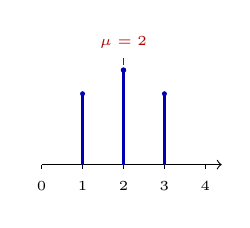
\begin{tikzpicture}[x=0.52cm,y=3.0cm]
              \draw[->,thin] (0,0) -- (4.4,0);
              \foreach \x in {0,1,2,3,4}
                \draw (\x,0) -- ++(0,-0.018) node[below=1pt] {\tiny \x};
              \draw[red!70!black,dashed] (2,0) -- (2,0.45);
              \node[red!70!black,above] at (2,0.45) {\tiny $\mu=2$};
              \draw[blue!70!black,line width=0.9pt] (1,0) -- (1,0.30);
              \draw[blue!70!black,line width=0.9pt] (2,0) -- (2,0.40);
              \draw[blue!70!black,line width=0.9pt] (3,0) -- (3,0.30);
              \fill[blue!70!black] (1,0.30) circle (0.9pt);
              \fill[blue!70!black] (2,0.40) circle (1.0pt);
              \fill[blue!70!black] (3,0.30) circle (0.9pt);
            \end{tikzpicture}
          \end{column}
        \end{columns}
        \vspace{0.5mm}
        Değerler ortalamaya daha \textbf{yakın} toplanır.
      \end{exampleblock}
    \end{column}
    \begin{column}{0.49\textwidth}
      \begin{exampleblock}{Şirket B (Daha Dağınık)}
        \footnotesize
        \begin{columns}[T,totalwidth=\linewidth]
          \begin{column}{0.52\linewidth}
            \centering
            \setlength{\tabcolsep}{2.7pt}
            \renewcommand{\arraystretch}{1.05}
            \begin{tabular}{cccccc}
              \toprule
              $x$ & 0 & 1 & 2 & 3 & 4 \\
              \midrule
              $f(x)$ & 0{,}2 & 0{,}1 & 0{,}3 & 0{,}3 & 0{,}1 \\
              \bottomrule
            \end{tabular}
          \end{column}
          \begin{column}{0.48\linewidth}
            \centering
            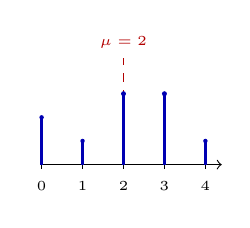
\begin{tikzpicture}[x=0.52cm,y=3.0cm]
              \draw[->,thin] (0,0) -- (4.4,0);
              \foreach \x in {0,1,2,3,4}
                \draw (\x,0) -- ++(0,-0.018) node[below=1pt] {\tiny \x};
              \draw[red!70!black,dashed] (2,0) -- (2,0.45);
              \node[red!70!black,above] at (2,0.45) {\tiny $\mu=2$};
              \draw[blue!70!black,line width=0.9pt] (0,0) -- (0,0.20);
              \draw[blue!70!black,line width=0.9pt] (1,0) -- (1,0.10);
              \draw[blue!70!black,line width=0.9pt] (2,0) -- (2,0.30);
              \draw[blue!70!black,line width=0.9pt] (3,0) -- (3,0.30);
              \draw[blue!70!black,line width=0.9pt] (4,0) -- (4,0.10);
              \fill[blue!70!black] (0,0.20) circle (0.8pt);
              \fill[blue!70!black] (1,0.10) circle (0.8pt);
              \fill[blue!70!black] (2,0.30) circle (0.9pt);
              \fill[blue!70!black] (3,0.30) circle (0.9pt);
              \fill[blue!70!black] (4,0.10) circle (0.8pt);
            \end{tikzpicture}
          \end{column}
        \end{columns}
        \vspace{0.5mm}
        Olasılık kütlesi ortalamadan \textbf{daha uzak} noktalara yayılır.
      \end{exampleblock}
    \end{column}
  \end{columns}

  \smallskip
  \footnotesize
  Sonuç: Ortalama aynı olsa bile, Şirket B'nin dağılımı daha geniştir; bu farkı ölçmek için \textbf{varyans} gerekir.
\end{frame}
\begin{frame}{İkonik Örnek: Kumarhanelerde Neden Bahis Limiti Var?}
    \begin{columns}[T]
        \begin{column}{0.70\textwidth}
        \justifying{}
        \small
        \textbf{Sıradışı Şans Senaryosu:} \\
        Düşünün ki o gün kumarhaneye gelen bir milyarder, tek bir ele 100~Milyon~TL yatırdı ve üst üste kazanarak inanılmaz şanslı bir seri yakaladı. Peki, kasanın her oyunda oyuncuya kaybettirme ihtimali daha yüksek olsa bile (beklenen değer kasanın lehine bile olsa), bu tek şanslı kişi kumarhaneyi batırabilir mi?

        \vspace{0.6em}
        \textbf{Varyans Riski:} \\
        Matematiksel beklenti uzun vadeyi garantiler. Fakat \textbf{Varyans}, kısa vadedeki aşırı dalgalanmaları ve "şans/risk" faktörünü ölçer. Çok yüksek miktarlı tek bir bahis masanın varyansını kasayı sarsacak seviyede yükseltir.

        \vspace{0.6em}
        \textbf{Sonuç ve Varyans Kontrolü:} \\
        Kumarhaneler kasayı batırmamak için oyunlara \textbf{Maksimum Masa Limiti} koyar. Bahisler limitlenerek varyans izole edilir (dalgalanma/şans riski azaltılır). Böylece oyunlar binlerce küçük bahse parçalanarak kasanın uzun vadede garanti parayı (ortalama getiri) alması mutlak şansa bırakılmadan netleştirilir.
        \end{column}
        \begin{column}{0.28\textwidth}
        \centering
        \includegraphics[width=\linewidth, keepaspectratio]{figures/roulette_expected_value.png}
        \end{column}
    \end{columns}
\end{frame}

\subsection{Varyansın Tanımı ve Hesaplanması}

\begin{frame}[fragile]
  \frametitle{Tanım 4.3 --- Varyans}
  Bir dağılımın değişkenliğini ölçmenin en yaygın yolu, gözlemlerin ortalamadan sapmalarının karesinin beklenen değerini almaktır.
  \begin{center}
    \begin{minipage}{0.95\textwidth}
      \begin{block}{Tanım 4.3 --- Varyans}
        Ortalaması $\mu$ ve dağılımı $f(x)$ olan $X$ rastgele değişkeninin \textbf{varyansı}:
        {\small
        \begin{align*}
          \sigma^2 &= E[(X-\mu)^2] = \sum_x (x-\mu)^2 f(x) \quad \text{(kesikli)} \\[4pt]
          \sigma^2 &= E[(X-\mu)^2] = \int_{-\infty}^{\infty} (x-\mu)^2 f(x)\,dx \quad \text{(sürekli)}
        \end{align*}
        }
        Gösterimler: $Var(X)$, $\sigma^2_X$ veya kısaca $\sigma^2$.
      \end{block}
    \end{minipage}
  \end{center}
  $(x - \mu)$ büyüklüğüne \textbf{sapma} (deviation) denir. Sapmalar karelenerek toplanıp ortalaması alındığı için, değerler $\mu$'ya yakınsa $\sigma^2$ küçük, uzaksa büyük olur.
\end{frame}

\begin{frame}[fragile]
  \frametitle{Örnek 4.8 --- Şirket A ve B Karşılaştırması}

  \smallskip
  Önceki slayttaki iki dağılımın varyanslarını hesaplayalım (her ikisinde de $\mu = 2{,}0$).

  \medskip
  \textbf{Şirket A:}
  {\small
  \begin{align*}
    \sigma^2_A &= (1-2)^2(0{,}3) + (2-2)^2(0{,}4) + (3-2)^2(0{,}3) = 0{,}6
  \end{align*}
  }

  \textbf{Şirket B:}
  {\small
  \begin{align*}
    \sigma^2_B &= (0-2)^2(0{,}2) + (1-2)^2(0{,}1) + (2-2)^2(0{,}3)\\
               &\quad + (3-2)^2(0{,}3) + (4-2)^2(0{,}1) = 1{,}6
  \end{align*}
  }

  \textbf{Sonuç:} $\sigma^2_B = 1{,}6 > \sigma^2_A = 0{,}6$. Şirket~B'nin araç kullanım sayısı çok daha \textbf{değişken} (variable).
\end{frame}

\begin{frame}[fragile]
  \frametitle[Teorem 4.2]{Varyansın Pratik Hesaplama Formülü}
  Her seferinde $(x - \mu)^2$ açılımını yapmak zahmetli olabilir. $(x-\mu)^2 = x^2 - 2\mu x + \mu^2$ açılarak toplam dağıtıldığında çok daha pratik bir formül elde edilir:

  \begin{center}
    \begin{minipage}{0.8\textwidth}
      \begin{block}{Teorem 4.2}
        \begin{center}
          $\sigma^2 = E(X^2) - \mu^2$
        \end{center}
      \end{block}
    \end{minipage}
  \end{center}

\end{frame}

\begin{frame}[fragile]
  \frametitle{Örnek 4.10 --- Kimyasal Reaktör Basınç Testi}

  \justifying{}
  \small \textbf{Vardiya Problemi:} Bir kimyasal tesisteki $X$ numaralı reaktörün \textbf{iç basınç endeksi} (milisaniye cinsinden dalgalanma payı) aşağıdaki yoğunluk fonksiyonu ile modellenmektedir. Buradaki $x = 1$ normal çalışma basıncını, $x = 2$ ise maksimum güvenli basıncı temsil eder. Endeksin $1$ ile $2$ arasında değiştiği ve grafiğinin aşağıdaki denklemle çalıştığı bilinmektedir:

  \vspace{0.5em}
  \begin{center}
    $f(x) = \begin{cases} 2(x-1), & 1 < x < 2 \text{ (Güvenli Dalgalanma Aralığı)} \\[2pt] 0, & \text{diğer durumlarda} \end{cases}$
  \end{center}

  \vspace{1em}
  \begin{exampleblock}{Mühendislik Görevi}
    \footnotesize Reaktörün ortalama basınç endeksini ($\mu$) ve bu basıncın reaktör çeperlerine yaptığı titreşim/değişkenlik stresini ölçmek için basınç varyansını ($\sigma^2$) mühendislik formülüyle hesaplayınız.
  \end{exampleblock}
\end{frame}

\begin{frame}[fragile]
  \frametitle{Örnek 4.10 --- Çözüm}

  \setbeamercovered{transparent=7}
  \uncover<2->{
    {\color{red!80!black}
    \justifying{}
    \footnotesize
    Ortalama ($\mu$) ve varyansı ($\sigma^2$) bulmak için Teorem 4.2'yi ($\sigma^2 = E(X^2) - \mu^2$) kullanacağız. Formül gereği integral hesabını iki aşamada yapmalıyız. 
    
    \vspace{0.4em}
    \scriptsize
    \textbf{Adım 1: Ortalama Basınç ($\mu$) Hesabı}
    \vspace{-0.8em}
    \begin{align*}
      \mu = E(X) &= \int_{1}^{2} x \cdot \underbrace{2(x-1)}_{f(x)}\,dx = 2\int_{1}^{2} (x^2 - x)\,dx \\[2pt]
                 &= 2 \left[ \frac{x^3}{3} - \frac{x^2}{2} \right]_{1}^{2} = 2 \left[ \left(\frac{8}{3} - \frac{4}{2}\right) - \left(\frac{1}{3} - \frac{1}{2}\right) \right] \\[2pt]
                 &= 2 \left[ \left(\frac{16-12}{6}\right) - \left(\frac{2-3}{6}\right) \right] = 2 \left[\frac{4}{6} - \left(-\frac{1}{6}\right)\right] = 2 \left(\frac{5}{6}\right) = \mathbf{\frac{5}{3} \approx 1{,}67}
    \end{align*}

    \vspace{0em}
    \textbf{Adım 2: Karelerin Beklenen Değeri ($E(X^2)$) Hesabı}
    \vspace{-0.8em}
    \begin{align*}
      E(X^2) &= \int_{1}^{2} x^2 \cdot 2(x-1)\,dx = 2\int_{1}^{2} (x^3 - x^2)\,dx \\[2pt]
             &= 2 \left[ \frac{x^4}{4} - \frac{x^3}{3} \right]_{1}^{2} = 2 \left[ \left(\frac{16}{4} - \frac{8}{3}\right) - \left(\frac{1}{4} - \frac{1}{3}\right) \right] = \mathbf{\frac{17}{6} \approx 2{,}83}
    \end{align*}

    \vspace{-0.8em}
    \textbf{Adım 3: Varyans ($\sigma^2$) Hesabı}
    \vspace{-0.8em}
    \begin{align*}
      \sigma^2 &= E(X^2) - \mu^2 = \frac{17}{6} - \left(\frac{5}{3}\right)^{\!2} = \frac{17}{6} - \frac{25}{9} = \frac{51 - 50}{18} = \mathbf{\frac{1}{18} \approx 0{,}056}
    \end{align*}
    }
  }
\end{frame}

\subsection{Standart Sapma}

\begin{frame}[fragile]
  \frametitle{Standart Sapma}
  Varyansın birimi, ölçülen büyüklüğün \textbf{karesidir} (örn.\ litre$^2$, TL$^2$). Doğrudan yorumlamak güçtür. Bu yüzden varyansın \textbf{pozitif karekökü} kullanılır:

  \begin{center}
    \begin{minipage}{0.8\textwidth}
      \begin{block}{Standart Sapma}
        \begin{center}
          $\sigma = \sqrt{Var(X)} = \sqrt{\sigma^2}$
        \end{center}
      \end{block}
    \end{minipage}
  \end{center}

  \begin{itemize}
    \item Standart sapma, değişkenle \textbf{aynı birime} sahiptir (litre, TL, saat vb.).
    \item Gözlemlerin ortalamadan \textbf{tipik olarak ne kadar saptığını} doğrudan gösterir.
  \end{itemize}
\end{frame}

% ─── SORULAR ─────────────────────────────────────
\subsection{Sorular}

\begin{frame}[fragile]
  \frametitle{Uygulama Görevi: Sunucu Yanıt Süresi (Sürekli)}
  \textbf{\small $\triangleright$~Sürekli Dağılımda İntegralle Varyans Hesabı}

  \smallskip
  \small
  Bir web sunucusunun yanıt süresi $X$ (ms) aşağıdaki olasılık yoğunluk fonksiyonu ile modellenmektedir:

  \[
    f(x) =
    \begin{cases}
      \dfrac{x}{8}, & 0 \le x \le 4, \\
      0,            & \text{diğer durumlarda.}
    \end{cases}
  \]

  \begin{block}{Görevler}
    \footnotesize
    \begin{enumerate}
      \item $f(x)$ fonksiyonunun geçerli bir yoğunluk olduğunu doğrulayınız: $\int_{-\infty}^{\infty} f(x)\,dx = 1$.
      \item Ortalama yanıt süresini bulunuz: $\mu = E(X) = \int_{0}^{4} x f(x)\,dx$.
      \item $E(X^2)$ ve varyansı hesaplayınız: $E(X^2) = \int_{0}^{4} x^2 f(x)\,dx$, $\sigma^2 = E(X^2) - \mu^2$.
    \end{enumerate}
  \end{block}

  \footnotesize
  Sonuçları kesirli ve yaklaşık ondalık değerlerle yazınız.
\end{frame}

\begin{frame}{Yazılım Kodu Hata Analizi}
  \textbf{\small $\triangleright$~Teorem~4.2 --- $\sigma^2 = E(X^2) - \mu^2$ Formulüyle Varyans Hesabı}

  \smallskip
  \small
  100 satırlık yazılım kodundaki yazım hatası sayısını temsil eden $X$ rastgele değişkeninin olasılık dağılımı aşağıda verilmiştir:

  \medskip
  \begin{center}
    \renewcommand{\arraystretch}{1.2}
    \begin{tabular}{cccccc}
      \toprule
      $x$ & 2 & 3 & 4 & 5 & 6 \\
      \midrule
      $f(x)$ & 0{,}01 & 0{,}25 & 0{,}40 & 0{,}30 & 0{,}04 \\
      \bottomrule
    \end{tabular}
  \end{center}

  \medskip
  \begin{block}{Görev}
    Teorem 4.2'yi ($\sigma^2 = E(X^2) - \mu^2$) kullanarak $X$'in \textbf{varyansını} hesaplayınız.
  \end{block}
\end{frame}

\begin{frame}{Yazılım Kodu Hata Analizi}
  \setbeamercovered{transparent=7}
  \uncover<2->{
    \small
    {\color{red!80!black}
      \textbf{Adım 1: Beklenen Değeri ($\mu$) Bulalım}
      \begin{align*}
        \mu = E(X) &= (2)(0{,}01) + (3)(0{,}25) + (4)(0{,}40) + (5)(0{,}30) + (6)(0{,}04) \\
             &= 0{,}02 + 0{,}75 + 1{,}60 + 1{,}50 + 0{,}24 = \mathbf{4{,}11}
      \end{align*}

      \textbf{Adım 2: $E(X^2)$ Değerini Bulalım}
      \begin{align*}
        E(X^2) &= (4)(0{,}01) + (9)(0{,}25) + (16)(0{,}40) + (25)(0{,}30) + (36)(0{,}04) \\
               &= 0{,}04 + 2{,}25 + 6{,}40 + 7{,}50 + 1{,}44 = \mathbf{17{,}63}
      \end{align*}

      \textbf{Adım 3: Varyansı Hesaplayalım}
      \begin{align*}
        \sigma^2 &= E(X^2) - \mu^2 \\
                 &= 17{,}63 - (4{,}11)^2 = 17{,}63 - 16{,}8921 = \mathbf{0{,}7379}
      \end{align*}
    }
  }
\end{frame}

\begin{frame}{Standart Sapma Hesabı}
  \textbf{\small $\triangleright$~Standart Sapma --- Varyansdan Karekök Alınması}

  \smallskip
  \small
  Bir $X$ rastgele değişkeninin olasılık dağılımı aşağıdaki şekilde tanımlanmıştır:

  \medskip
  \begin{center}
    \renewcommand{\arraystretch}{1.2}
    \begin{tabular}{cccc}
      \toprule
      $x$ & $-2$ & 3 & 5 \\
      \midrule
      $f(x)$ & 0{,}3 & 0{,}2 & 0{,}5 \\
      \bottomrule
    \end{tabular}
  \end{center}

  \medskip
  \begin{block}{Görev}
    $X$ değişkeninin \textbf{standart sapmasını} bulunuz.
  \end{block}
\end{frame}

\begin{frame}{Standart Sapma Hesabı}
  \setbeamercovered{transparent=7}
  \uncover<2->{
    \small
    {\color{red!80!black}
      \textbf{Adım 1: $\mu$ ve $E(X^2)$ Hesabı}
      \begin{align*}
        \mu = E(X) &= (-2)(0{,}3) + (3)(0{,}2) + (5)(0{,}5) \\
                   &= -0{,}6 + 0{,}6 + 2{,}5 = \mathbf{2{,}5} \\[6pt]
        E(X^2) &= (4)(0{,}3) + (9)(0{,}2) + (25)(0{,}5) \\
               &= 1{,}2 + 1{,}8 + 12{,}5 = \mathbf{15{,}5}
      \end{align*}

      \textbf{Adım 2: Varyans ve Standart Sapma}
      \begin{align*}
        \text{Varyans } (\sigma^2) &= 15{,}5 - (2{,}5)^2 = 15{,}5 - 6{,}25 = \mathbf{9{,}25} \\[6pt]
        \text{Standart Sapma } (\sigma) &= \sqrt{9{,}25} \approx \mathbf{3{,}041}
      \end{align*}
    }
  }
\end{frame}
% ────────────────────────────────────────────────────────────────

\section{Beklenen Değerin Özellikleri}
\subsection{Temel Özellikler}

\begin{frame}[fragile]
  \frametitle{Teorem 4.5 --- Doğrusal Dönüşüm}
  Beklenen değerleri her seferinde tanımdan hesaplamak yerine, aşağıdaki güçlü özellikler kullanılır.
  \begin{center}
    \begin{minipage}{0.9\textwidth}
      \begin{block}{Teorem 4.5}
        $a$ ve $b$ sabit sayılar olmak üzere:
        \begin{center}
          $E(aX + b) = a\,E(X) + b$
        \end{center}
      \end{block}
    \end{minipage}
  \end{center}

  \medskip
  \textbf{Özel durumlar (Sonuçlar):}
  \begin{itemize}
    \item $a = 0$ ise: $E(b) = b$ \quad (Sabitin beklenen değeri kendisidir.)
    \item $b = 0$ ise: $E(aX) = a\,E(X)$ \quad (Sabit çarpan dışarı çıkar.)
  \end{itemize}
\end{frame}

\begin{frame}[fragile]
  \frametitle[Örnek 4.17]{Örnek 4.17 --- Teorem 4.5 Uygulaması}

  \smallskip
  \textbf{Soru:} Otopark yıkayıcısı örneğinde görevlinin geliri $g(X) = 2X - 1$ idi. Teorem~4.5 ile $E(2X - 1)$ değerini bulunuz.

  \medskip
  \textbf{Çözüm:} Teorem~4.5'e göre: $E(2X - 1) = 2\,E(X) - 1$.

  Daha önce doğrudan hesaplayarak $E(X) = \frac{41}{6}$ bulmuştuk.
  \begin{align*}
    E(2X - 1) &= 2\left(\frac{41}{6}\right) - 1 = \frac{41}{3} - 1 = \$12{,}67
  \end{align*}
  Aynı sonuca, Teorem~4.1 ile uzun yoldan da ulaşmıştık. Teorem~4.5 işlemi \textbf{kısaltır}.
\end{frame}

\begin{frame}[fragile]
  \frametitle{Teorem 4.6 --- Toplam ve Farkın Beklenen Değeri}
  \begin{center}
    \begin{minipage}{0.95\textwidth}
      \begin{block}{Teorem 4.6}
        Bir rastgele değişkenin iki veya daha fazla fonksiyonunun toplam/farkının beklenen değeri, beklenen değerlerin toplam/farkına eşittir:
        \begin{center}
          $E[g(X) \pm h(X)] = E[g(X)] \pm E[h(X)]$
        \end{center}
      \end{block}
    \end{minipage}
  \end{center}

  \medskip
  Bu özellik iki ayrı rastgele değişken olan $X$ ve $Y$ için de geçerlidir (Sonuç~4.4):
  \begin{center}
    $E(X \pm Y) = E(X) \pm E(Y)$
  \end{center}

  {\small \textbf{Yorum:} $X$, A makinesinin günlük üretimi ve $Y$, B makinesinin günlük üretimi ise $E(X+Y)$, iki makinenin \textbf{toplam} ortalama üretimine eşittir.}
\end{frame}

\begin{frame}[fragile]
  \frametitle[Örnek 4.19]{Örnek 4.19 --- Teorem 4.6 Uygulaması}

  \smallskip
  \textbf{Soru:} $X$'in dağılımı: $f(0)=\tfrac{1}{3}$, $f(1)=\tfrac{1}{2}$, $f(2)=0$, $f(3)=\tfrac{1}{6}$. \; $E[(X-1)^2] = ?$

  \medskip
  \textbf{Çözüm:} Teorem~4.6 ile $(X-1)^2 = X^2 - 2X + 1$ açılır:
  \begin{center}
    $E[(X-1)^2] = E(X^2) - 2\,E(X) + E(1) = E(X^2) - 2\,E(X) + 1$
  \end{center}

  {\small
  \begin{align*}
    E(X) &= (0)\!\left(\tfrac{1}{3}\right) + (1)\!\left(\tfrac{1}{2}\right) + (2)(0) + (3)\!\left(\tfrac{1}{6}\right) = 1 \\[4pt]
    E(X^2) &= (0)\!\left(\tfrac{1}{3}\right) + (1)\!\left(\tfrac{1}{2}\right) + (4)(0) + (9)\!\left(\tfrac{1}{6}\right) = 2
  \end{align*}
  }
  \begin{center}
    $E[(X-1)^2] = 2 - 2(1) + 1 = \mathbf{1}$
  \end{center}
\end{frame}

\subsection{Birden Fazla Değişken}

\begin{frame}[fragile]
  \frametitle{Teorem 4.8 --- Bağımsız Değişkenlerin Çarpımı}
  Toplam/fark için bağımsızlık şartı gerekmezken, \textbf{çarpım} söz konusu olduğunda durum farklıdır:
  \begin{center}
    \begin{minipage}{0.9\textwidth}
      \begin{block}{Teorem 4.8}
        $X$ ve $Y$ \textbf{istatistiksel olarak bağımsız} ise:
        \begin{center}
          $E(XY) = E(X) \cdot E(Y)$
        \end{center}
      \end{block}
    \end{minipage}
  \end{center}

  \medskip
  \begin{itemize}
    \item Örneğin yeşil ve kırmızı zarlar atıldığında, zarlar birbirinden bağımsız olduğu için zarların çarpımının beklenen değeri, her birinin beklenen değerlerinin çarpımına eşittir.
    \item \textbf{Sonuç 4.5:} $X$ ve $Y$ bağımsız ise kovaryansları sıfırdır: $\sigma_{XY} = 0$.
  \end{itemize}
\end{frame}

% ─── SORULAR ─────────────────────────────────────
\subsection{Sorular}

\begin{frame}{Doğrusal Dönüşüm}
  \textbf{\small $\triangleright$~Teorem~4.5 --- Doğrusal Dönüşümde Beklenen Değer ve Varyans}

  \smallskip
  \small
  Daha önce (Teorem~4.2 ile Varyans sorusunda) 100 satırlık yazılım kodundaki hata sayısını temsil eden $X$ rastgele değişkeni için şu değerleri bulmuştuk:
  \begin{center}
    $E(X) = 4{,}11 \quad \text{ve} \quad Var(X) = 0{,}7379$
  \end{center}

  \begin{block}{Görev}
    $Z = 3X - 2$ formülü ile tanımlanan rastgele değişken $Z$'nin:
    \begin{enumerate}
      \item[(a)] Beklenen değerini hesaplayınız.
      \item[(b)] Varyansını hesaplayınız.
    \end{enumerate}
  \end{block}
  \vspace{0.2cm}
  {\footnotesize \textit{Kaynak: Walpole, Bölüm 4, Alıştırma 4.53 \cite{walpole_ch4}}}
\end{frame}

\begin{frame}{Doğrusal Dönüşüm}
  \setbeamercovered{transparent=7}
  \uncover<2->{
    \small
    {\color{red!80!black}
      \textbf{(a) Beklenen Değer (Teorem 4.5):}
      \begin{align*}
        E(Z) &= E(3X - 2) \\
             &= 3\,E(X) - 2 \\
             &= 3(4{,}11) - 2 = 12{,}33 - 2 = \mathbf{10{,}33}
      \end{align*}

      \textbf{(b) Varyans (Sonuç 4.6, 4.8):}
      \begin{align*}
        Var(Z) &= Var(3X - 2) \quad \text{(sabit terim varyansı etkilemez)}\\
               &= Var(3X) \\
               &= 3^2\,Var(X) \\
               &= 9\,(0{,}7379) = \mathbf{6{,}6411}
      \end{align*}
    }
  }
\end{frame}

% ────────────────────────────────────────────────────────────────

\section{Özet}

\begin{frame}[fragile]
  \frametitle{Genel Özet (Bölüm 1)}
  \begin{center}
    \renewcommand{\arraystretch}{1.4}
    {\small
    \begin{tabular}{p{4.5cm}p{6.5cm}}
      \toprule
      \textbf{Kavram} & \textbf{Formül / Not} \\
      \midrule
      Beklenen Değer (kesikli) & $\mu = E(X) = \sum_x x\,f(x)$ \\
      Beklenen Değer (sürekli) & $\mu = E(X) = \int x\,f(x)\,dx$ \\
      \midrule
      Varyans & $\sigma^2 = E(X^2) - \mu^2$ \\
      Standart Sapma & $\sigma = \sqrt{\sigma^2}$ \; (aynı birim) \\
      \bottomrule
    \end{tabular}
    }
  \end{center}
\end{frame}

\begin{frame}[fragile]
  \frametitle{Genel Özet (Bölüm 2)}
  \begin{center}
    \renewcommand{\arraystretch}{1.4}
    {\small
    \begin{tabular}{p{4.5cm}p{6.5cm}}
      \toprule
      \textbf{Kavram} & \textbf{Formül / Not} \\
      \midrule
      $E(aX + b)$ & $= a\,E(X) + b$ \\
      \midrule
      $E(X \pm Y)$ & $= E(X) \pm E(Y)$ \; (her zaman) \\
      $E(XY)$ & $= E(X)\,E(Y)$ \; (bağımsızsa) \\
      \bottomrule
    \end{tabular}
    }
  \end{center}
\end{frame}

\begin{frame}[allowframebreaks]
  \frametitle{Kaynaklar}
  \nocite{walpole_ch4}
  \printbibliography{}
\end{frame}

\appendix

\section{Yapay Zeka Asistanı}
\begin{frame}{Yapay Zeka Asistanınız: NotebookLM}
    \begin{columns}[T]
        \begin{column}{0.48\textwidth}
            \justifying{}
            \textbf{Ders Materyalleri ile Etkileşime Geçin!}

            Bu dersin tüm içeriği (sunumlar, makaleler ve notlar), Google'ın gelişmiş yapay zeka asistanı \textbf{NotebookLM} sistemine yüklenmiştir.

            \vspace{1em}
            \begin{itemize}
                \item \textbf{Anında Cevaplar:} Aklınıza takılanları sorun.
                \item \textbf{Özetler:} Karmaşık konuları basitçe öğrenin.
                \item \textbf{Audio Overview:} Dersi bir podcast gibi dinleyin.
            \end{itemize}

            \vspace{1.5em}
            \begin{center}
                {\setbeamercolor{button}{bg=red,fg=black}
                \href{https://notebooklm.google.com/notebook/1daaa713-b9d0-4bb3-bbe6-defbaf4e67d4}{\beamerbutton{\rule[-4ex]{0pt}{11ex}\Large \textbf{Hemen Deneyin}}}}
            \end{center}
        \end{column}

        \begin{column}{0.48\textwidth}
            \centering
            \includegraphics[width=\textwidth, height=0.6\textheight, keepaspectratio]{figures/notebooklm.jpg}
        \end{column}
    \end{columns}
\end{frame}

\begin{frame}[plain,noframenumbering]
    \begin{tikzpicture}[remember picture,overlay]
        \node[anchor=center, at=(current page.center), inner sep=0pt] {
            \includegraphics[width=\paperwidth, height=\paperheight]{figures/combined_qrs.png}
        };
        \node[anchor=south, at=(current page.south), yshift=0.5cm, fill=white!95, rounded corners, inner sep=10pt, text width=0.95\paperwidth, align=center] {
            \Large \textbf{\textcolor{blue}{Bizi Takip Edin!}} \\
            \vspace{0.3em}
            \small Ders tekrarlarıyla konuları pekiştirmek (YouTube), profesyonel proje ağlarına katılmak (LinkedIn) ve kampüs duyurularından anında haberdar olmak (Instagram) için topluluğumuza katılın.
        };
    \end{tikzpicture}
\end{frame}

\end{document}
